%--- Chapter 4 ----------------------------------------------------------------% 
\chapter{Methodology}  \label{ScalabilityModel}

In the previous chapters, we gave a short synopsis of what the framework tries to achieve and why we need it. We also briefly discussed the supporting concepts required for understanding the framework. In this chapter, we describe the in-depth concepts behind the framework along with explaning why we implemented a particular technique and all the other alternative techniques that we tried or contemplated trying. Although this chapter covers details about all implementations and techniques we tried, information on why some of the methods failed or problems with implementations are discussed in the results and analysis section. 

We have previously mentioned that our framework provides selection techniques for two broad classes of problems, namely, parallel graph processing and system of linear equations. To maintain the specified structure, this chapter will be sub-categorized into each of those problems. 

\section{Selection of parallel graph processing packages}
It has already been established that with a plethora of available parallel graph processing packages, selection based on hard empirical evidence of various experiments are time and resource consuming to obtain and as a result, we are introducing machine learning based package selection. In terms of what we can achieve with a machine learning based framework for package selection, we could either perform execution time prediction or a binary classification of packages for a particular graph and hardware features. Hence, this section is further categorized into two subsections, with each detailing one of the aspects. 


\subsection{Execution time prediction of graph processing experiments}
The objective here is to efficiently and accurately predict the execution time of a particular experiment without explicitly running those experiments. An experiment in this context is one specific package running one specific algorithm over one specific graph dataset across given hardware configurations.

Machine learning-based projects differ from each other in various ways, but the two universally common requirements is a dataset and a model. To distinguish between a machine learning dataset and graph dataset, throughout this thesis, we would be referring to the former as a learning set and the actual graph dataset as a dataset.

The learning set in this case is a collection of individual runs of experiments which consists of three tangible elements, i.e.) dataset, algorithm, and package along with its features and ground truth. The dataset is any graph dataset in edge-view format. Datasets come in two flavors. One is a synthetic dataset which we auto-generated \todo{background}. We use the Graph500 synthetic graph generator which creates a Kronecker graph with initial parameters of A = 0.57, B = 0.19, C = 0.19, and $D = 1 − (A + B + C) = 0.05$ and set the average degree of a vertex as 16. Hence, a Kronecker graph with scale S has $2^S$ vertices and approximately $16 * 2^S$ edges. Kronecker graphs are a generalization of RMAT graphs. The RMAT takes the scale as a parameter. Most of our experiments have a scale of 22, which is 4,194,304 vertices and an average of 16 edges per vertex. 

Another flavor of the dataset is real-world dataset. These are the graph datasets that that are modeled from real-world applications like connectivity map of Facebook and Google. These real-world datasets are obtained from scraping the web sources using Beautiful soup. The web sources include SNAP and Konect databases\todo{background}. Overall, we have managed to get 450 different graph datasets that are a combination of real-world and synthetic graphs.

The next tangible element is the algorithm. In our framework, a list of four algorithms which includes breadth-first search(BFS), triangle count(TC), single source shortest path(SSSP), and page rank(PR)\todo{background} is implemented on each dataset. More details on these algorithms are explained in the background section. Each of these algorithms is performed by six different parallel graph processing packages that include GAP, GraphMat, Graph500, GraphBig, Galois, and Powergraph, which are again explained in detail in the background section.

\begin{figure*}
    \centering
    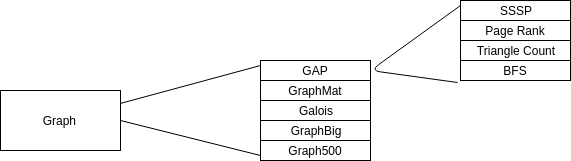
\includegraphics[width=1\columnwidth]{figures/dataset_flow.png}
    \caption{Multiple levels of abstractions in the learning set}
    \label{dataset_flow}
\end{figure*}

\subsubsection{Learning set}
Figure ~\ref{dataset_flow}  shows us the multilevel abstraction in our learning set, where each graph dataset has four possible algorithms, and six different graph processing packages can implement each algorithm. As a result, 24 different experiments need to be conducted for each graph dataset bringing our total experiment count to 4000, which is the size of our learning set. Each experiment in the learning set is accompanied by the features of the graph and its ground truth value, which in this case is the execution time of that particular experiment.  

Since different algorithms have different execution times, it won't really be fair if we trained our model across all algorithms. For this purpose we also filter the datapoints with respect to each algorithm. The learning set with the first 10 entries can be seen in figure \ref{learning set} 

\begin{figure*}
    \centering
    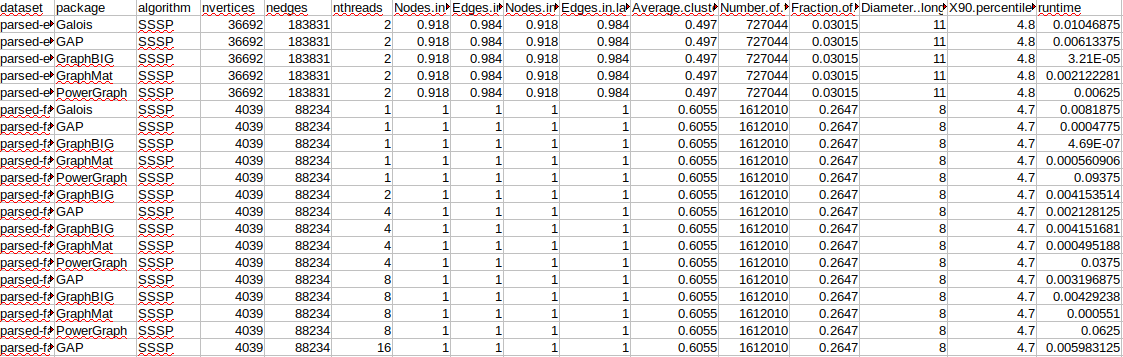
\includegraphics[width=1\columnwidth]{figures/learning_set.png}
    \caption{First 20 rows of learning set}
    \label{learning set}
\end{figure*}
\subsubsection{Feature selection}
The metadata of each experiment acts as the features upon which a prediction model is implemented. The features are a mix of both metadata of the graph by itself and hardware configurations. Based on regression analysis, the 12  features that had coefficients above 0.2 were finally chosen in the learning set. Features with high coefficients signify high correlation with execution time and are more likely that they would contribute more towards an accurate prediction by the model. The first three features with the highest coefficients are physical properties of the graph and hardware:

\begin{enumerate}
  \item Number of vertices
  \item Number of edges
  \item Number of Threads
\end{enumerate}
The number of vertices has a correlation coefficient of 0.86 towards influencing the execution time. This is quite straightforward as execution time is largely dependent on the size of the graph.

Consequently, so is the number of edges with a coefficient of 0.81. The number of threads follows behind with a coefficient of 0.77 as it determines the communication complexity and time lost in transferring data. The next set of features relates to the density and connectivity of the graph: 

\begin{figure*}
    \centering
    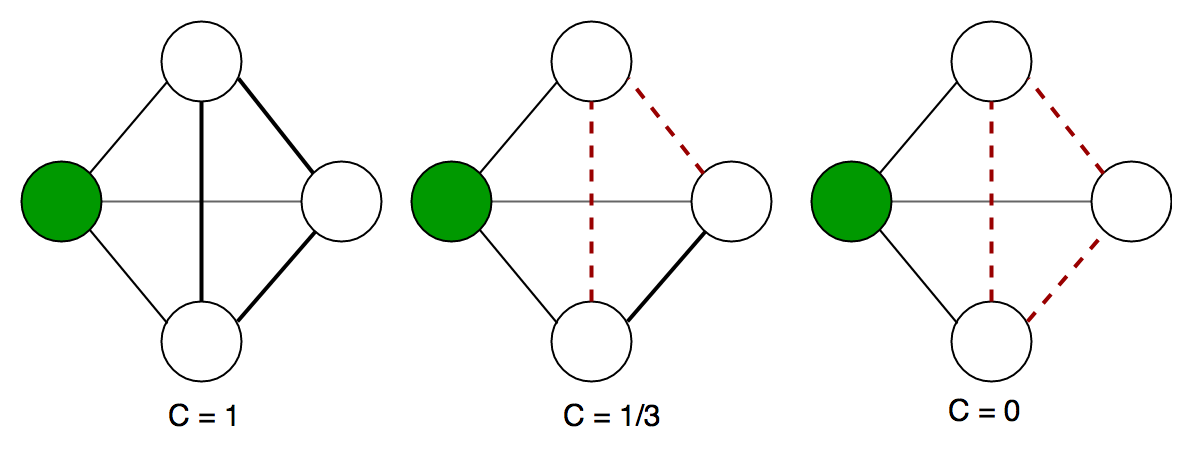
\includegraphics[width=1\columnwidth]{figures/features_avg_clustering.png}
    \caption{Average clustering coefficient}
    \label{Average clustering coefficient}
\end{figure*}

\begin{figure*}
    \centering
    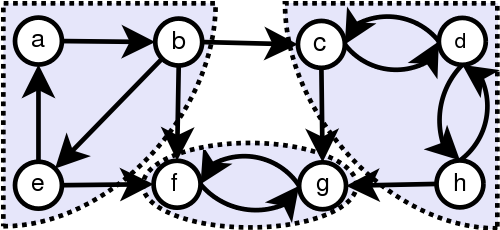
\includegraphics[width=.5\columnwidth]{figures/features_scc.png}
    \caption{Connected components}
    \label{Connected components}
\end{figure*}


\textbf{Average clustering coefficient}\\
The clustering coefficient is a measure of how well the neighbors of a node are connected. ~\ref{Average clustering coefficient}  depicts an example calculation of the clustering coefficient. The local clustering coefficient of the green node is computed as the proportion of connections among its, which are realized compared with the number of all possible connections. In the figure, the green node has three neighbors, which can have a maximum of 3 connections among them. In the left part of the figure, all three possible connections are realized (thick black segments), giving a local clustering coefficient of 1. In the middle part of the figure, only one connection is realized (solid black line), and two connections are missing (dotted red lines), giving a local cluster coefficient of 1/3. Finally, none of the possible connections among the neighbors of the green node are realized, producing a local clustering coefficient value of 0. The average across all nodes in the graph gives an average clustering coefficient.  This feature has a correlation coefficient of 0.67.

\textbf{Nodes and edges in largest connected components}\todo{rework}\\
A set of nodes are said to be strongly connected if there is a path between all pairs of nodes within the set. In figure ~\ref{Connected components}, it can easily be seen there are three strongly connected components(SCC). The number of nodes in the largest SSC tells us how big the most connected part of the graph is. This feature has a correlation coefficient of 0.61 towards execution time. Likewise, a set of nodes are said to be weakly connected if there is any path regardless of direction between all pairs of nodes within the set. In the same figure ~\ref{Connected components}, all of the nodes belong to one large weakly connected component as there exist some path between all pairs of nodes which doesn't necessarily need to be direct like SCC. This feature has a correlation coefficient of 0.52.

\textbf{Number of triangles and fraction of closed triangles}\\
A triangle is three nodes that are connected by either two (open triangle) or three (closed triangle) undirected ties. The fraction of closed triangle is the ratio of closed triangles to the total number of triangles. The number of triangles has a correlation coefficient of 0.44, while the fraction of closed triangles has a correlation coefficient of 0.48. \\

\textbf{Diameter and effective diameter}\\
The diameter of a graph is the maximum eccentricity of any vertex in the graph. That is, it is the greatest distance between any pair of vertices. To find the diameter of a graph, first, find the shortest path between each pair of vertices. The greatest length of any of these paths is the diameter of the graph. The effective diameter is the shortest hops in which 90\% of the nodes are covered. They have a correlation coefficient of 0.32 and 0.39, respectively. 

The graph density based features tend to have a high correlation to the execution time as they determine the number of iterations for the algorithms we chose. More iterations correspond to more execution time. 

Apart from these features, other graph properties were not selected as their correlation coefficient was less than 0.3, which we used as a threshold for selected features. These include :
\begin{itemize}
    \item \textbf{Wedge count} - A wedge is defined as a path with two hops. A triangle has 3 possible wedges.
    \item \textbf{Square count} - Similar to triangles, a square is a closed loop enclosed by 4 edges.
    \item \textbf{Fill} - It is a metric to measure the fraction of existing edges to total number of possible edges
    \item \textbf{Spectral norm} - It is the largest absolute eigenvalue of the graph's adjacency matrix.
\end{itemize}



\subsubsection{Prepossessing}
Although we have learning set with graph data, hardware configurations, and its execution time as ground truth, it is still not ready for a model to be trained on. That requires a series of additional prepossessing steps to clean the learning set fully. The prepossessing steps in its respective order are: 

\textbf{Removing noise}\\
The most basic step in any data cleaning is removing noise. A noise comes in multiple types, but the most common type is missing features. For synthetic datasets, this isn't a problem as all the features are manually generated, and as a result, we have control over what features are needed. But for real-world graphs, this can be a problem as we scrubbed the features provided by SNAP and Konect for each of its datasets. Since we are getting our real-world graphs from two different sources, the features provided don't necessarily match. One such example is the wedge count feature. Konect offers wedge count for its datasets, but SNAP doesn't. Hence we had to interpolate wedge count for the experiments with SNAP dataset or drop those points entirely from the learning set. Dropping data points mean a smaller learning set, and since we already don't have too many points to spare, we resort to imputing those missing values rather than dropping them. 

In general, there are some excellent multi-feature imputers available, but since only a fraction of experiments uses Konect datasets, a simple imputer does fine with this learning set. The sklearn's simple imputer uses one of three methods to fill missing, ie) mean, median, mode while for our framework, we used a simple imputer with median fill. 

Another typical flavor of noise comes from features that have infinity as its value. This mostly occurs for features that rely on convergence for its final values. During feature computation, when models don't converge, it sets its default value as float max, which can be considered as infinity. The only way to handle data points with unconverged features is to drop that data point entirely. But on a positive note, we ended up losing only ~30 data points due to unconverged data.

\textbf{Feature normalization}\\
Another important step for accurate predictions is for all the features to be scaled within the same range. Before normalization, different features have values in different ranges. For example, the value of the average clustering coefficient ranges between 0 and 1, while the number of edges and vertices are absolute counts. An ideal normalization would be to scale down all features between 0 and 1. For this purpose we use min-max scaling\todo{background}.

\textbf{Converting nominal data to numeric}\\
Learning set columns like algorithm and package have nominal categorical data but using a regression model(discussed ahead in the section) requires only numeric data, so we assign a unique numeric value to each category within a feature column. For example, there are four different algorithms; hence, we assign them unique values between 0 and 3. Likewise, we also assign values for the six packages.

\textbf{1-hot encoding}\\
Now that the categorical data have been assigned numeric values, this promotes a new problem where the model doesn't recognize it as categorical data and treats those feature to scale rather than taking it for its face value. By not doing so, the value of category influences the weights assigned to features. For example, we have assigned the package GAP with category 2 and Galois with category 3. Although there is no underlying significance of the category number, the model treats Galois better than GAP. 

To avoid this, we encode the category into a 1-hot vector where the position in a vector addresses each category with its size being the number of categories. Figure \ref{Example of 1-hot encoding} gives us an excellent example of how 1-hot encoding is done.


\begin{figure*}
    \centering
    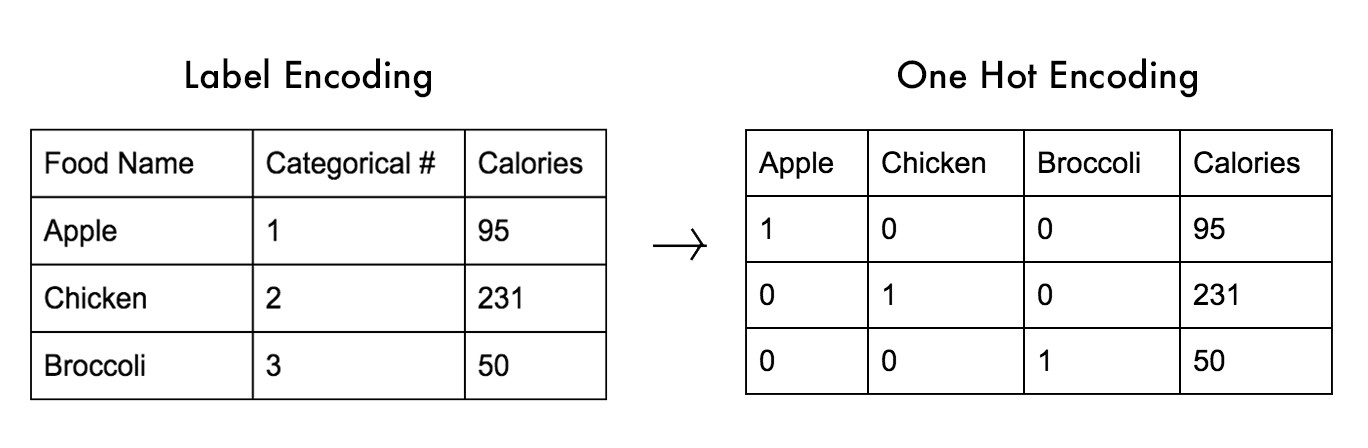
\includegraphics[width=1\columnwidth]{figures/preprocess_1_hot.jpeg}
    \caption{Example of 1-hot encoding}
    \label{Example of 1-hot encoding}
\end{figure*}
\todo{Give table with actual example}

\subsubsection{Fitting the model}
After complete prepossessing, the learning set is ready for training. In this thesis, we will discuss four different configurations of models used with each one slightly tuned based on the previous. Results from each configuration and its analysis are discussed in the next chapter. \\

\begin{enumerate}
    \item Linear regression with unnormalized learning set
    \item Linear regression with normalized learning set
    \item Ridge regression with unnormalized learning set
    \item Ridge regression with normalized learning set
\end{enumerate}
 

By analyzing the data points, one can see that they are not linearly separable. But going ahead in that direction, we initially tried using linear regression. Before exploring options for normalizing the learning set, we wanted to see how the models fared on raw data to identify new strengths and weakness of each. The configurations with unnormalized learning set include features that aren't scaled to a 0-1 range.

Another problem we notice after analyzing the learning set is that the features undergo the phenomenon of multicollinearity. A collection of features are said to be multicollinear if they are linearly proportional to each other to a certain extent. In that case, the features can derive themselves from each other. This creates a problem as the main objective of regression analysis is to isolate independent features from each other and tune one feature at a time until predictions improve with keeping other features constant and thus finding the relationship between the dependent and independent features. But it's hard to estimate this relationship if the independent features change in unison. 


For example, the synthetic graphs are generated with 16 edges per vertex on an average. As a result, the number of edges can be linearly derived to a certain extent from the number of vertices. Dropping one of these features is also not an option as when dealing with execution times in such small margins, the minor differences in the size of the graph contribute significantly towards the final predictions.

To solve this problem, we went ahead with using a ridge regression model, which is a class of regression that uses l2 regularization. Here the size of coefficients is limited by adding a penalty equalling the square of the magnitude of coefficients. To simplify, it adds a bias to each feature to avoid division by zero encountered by multicollinear features. Ridge regression on normalized and unnormalized learning sets make up the last two configurations. More on ridge regression and multicollinearity is given in the background section.

\subsubsection{Experiments and Validation}
To validate the accuracy of the model, the learning set is further divided into training and testing set. The split in data points consists of a 70\% allocation to training set and 30\% allocation to the testing set from a total of 4000 data points. This is done by Sklearn's test\_train\_split() with splits into random test-train subsets. 

\todo{More on where the experiments were run(Talapas) and cost of feature extraction(Need to verify with Sam }

\subsection{Classification of graph processing experiments}\\ \todo{The learning set and the features are the same. Hence I will bring those out with prediction and classification as subsections.}\\
Predictive modeling of execution time is great, but interpreting and coming to a conclusion with such small values can be challenging. Minor inaccuracies in predictions will significantly add up across the course of an application running thousands of experiments. But instead, a user would greatly benefit if he knows if a specific package is worth using for a particular experiment. For this reason, we have implemented a classification framework that predicts a binary class label of "good" or "bad" based on the features of the graph dataset and hardware configurations.  

\subsubsection{Preprocessing}
To perform classification, we must perform the same preprocessing steps as the regression framework except for converting nominal to numeric. Apart from that, we must also add a class label for training. \\
\textbf{Traversed edges per second}\\
We could use execution time solely as the metric for classifying between a good and bad experiment, but that wouldn't take the size of graph datasets into account. To use an appropriate metric that scales with the size of the dataset and is also a function of execution time, we use traversed edges per second(TEPS) as a metric for classification. TEPS is defined by :


    $TEPS= \dfrac{Number\;of\; edges}{Execution\;time}$ \\


TEPS is a useful metric for this problem as it not only scales with execution time but also captures both the computational and communication capabilities of the experiment and hardware. One must note that lower TEPS indicates better performance as it's a factor of execution time rather than a multiple of it. 

\textbf{Binary label classification}\\
For this framework, we decided to use a binary classification of "good" and "bad" for a particular experiment based on the TEPS value. For any experiment n, it's binary class label could be defined as:


\[
  label(n) =
  \begin{cases}
                                   good & \text{, if $x < 2/3((\sum_{n=1}^{N} x_{n} )/N)$} \\
                                   bad & \text{, if $x > 2/3((\sum_{n=1}^{N} x_{n} \ )/N)$} \\
  \end{cases}
\]
 ,where N is the number of experiments in the learning set and x is the TEPS value of a particular experiment. Intuitively, this function classifies an experiment as "good" if it has a TEPS value of less than 2/3 times the mean across all the TEPS values in the learning set and "bad" otherwise. This split approximately labels 30\% of the learning set as "good" and 70\% as "bad"
   
\subsubsection{Classification model}
Similar to predictive modeling, we will have two configurations of models with the latter improving upon the former. 


\begin{enumerate}
    \item Logistic regression with normalized learning set
    \item Random forest with normalized learning set
\end{enumerate}
Even though it was established that the learning set is not linearly separable, our first model is logistic regression just for the sake of comparison with our random forest model. \todo{background}More details on the two models are given in the background section.\\

\subsubsection{Experiment and validation}
\todo{same as before}

\todo{need to work on the transition. Seems a bit sudden}
\section{Selection of solvers for a system of linear equations}
\\For any software selection framework, a classification model based on performance is a great first step, but a binary classification has significant drawbacks on its own. First off, users need to provide their choice of package for which the framework will classify as "good" or "bad" based on the experiment setup. This is added work for a user who doesn't really care about the package and wants a good one to use. But more importantly, a binary classifier may yield a lot of possible good packages giving the user further decisions to make, thereby defeating the primary purpose of this framework. It would be a significant improvement if the framework could provide what the best package would be for that experiment. Or better yet, a ranked list of packages for that experiment.

\subsection{Ranking framework}
To achieve the goal mentioned above, we look at a different class of application to the previous graph processing one. Specifically, we aim to provide a framework that gives a ranked list of linear solvers for a system of linear equation.

\subsubsection{Learning set}
Similar to the previous application, this also contains experimental setup along with its features and ground truth value as data points of the learning set. The experimental setup, in particular, is a system of linear equation in the form of matrix A and right-hand vector B together represented as system M.\todo{Verify} Each system M has a list of solvers and preconditioners.\todo{Background} Figure\todo{add similar figure} shows us an abstraction of the learning set with each unique system-solver combination as an experiment and thereby a data point. 

With establishing the setup of learning set, we move on to the two categories of experiments run, with each having one learning set.\todo{ Two paragraphs for Moose and UFL}

\subsubsection{Feature selection}

\begin{enumerate}
    \item Trace and absolute trace
    \item Column diagonal dominance
    \item Dimension
    \item Diagonal mean
    \item Frobenius norm
\end{enumerate}
\todo{Explanation for each }

\subsubsection{Two stage ranking algorithm}
After analyzing the results of both classification and predictive modeling, both of which are discussed in the next chapter, we provide a ranking algorithm that tries to benefit from the unique advantages that both offer on the learning set. 



The basic idea behind this algorithm is the fact prediction works better on data that has been classified "good" or "bad". When the class label is added as an additional feature for predictive modeling, the quality of predictions improve. The two stages refer to the two models for classification and prediction being used by the algorithm. With a reasonable enough prediction accuracy of execution time for different experiments, they could potentially be sorted to give a good ranked list of solvers that work best for a particular system of linear equations. Figure \ref{Overview of the ranking algorithm} provides us with the workflow of the two-stage algorithm.


\begin{figure*}
    \centering
    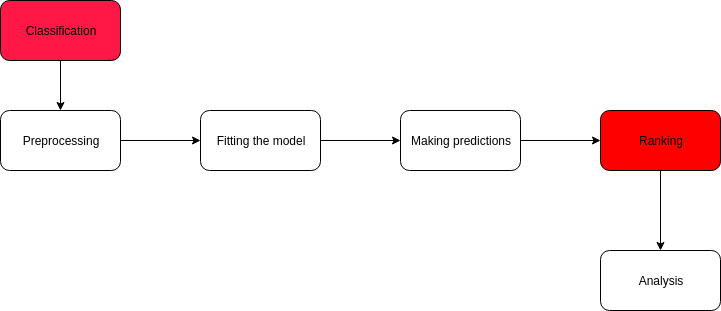
\includegraphics[width=1\columnwidth]{figures/ranking_overview.png}
    \caption{Overview of the ranking algorithm}
    \label{Overview of the ranking algorithm}
\end{figure*}
\todo{similar diagram but classification comes after prepossessing}

\textbf{Preprocessing}\\
\todo{My prepossessing is more or less the same as before but need to check with Kanika}
\textbf{Classification}\\
%I will just do 1 paragraph about it as I blindly assume the labels come from the C4.5 algorithm with very good accuracy. Will cite Kanika's paper%

\textbf{Fitting the model and hyperparameters}
After classification, the learning set with a "good" or "bad" class label is ready for predictive modeling. By analyzing the results from predictive modeling in the graph processing application, We decided to use the final model configuration that uses ridge regression on the normalized dataset. A detailed description of the hyperparameters are given the background section.\todo{background} Hyperparameter tuning was done with the help of 5-fold cross-validation. After tuning, the best set values for hyperparameters were:\\

\begin{enumerate}


    \item \textbf{Regularization strength}
Since ridge regression uses L2 regularization, a regularization strength must be provided. After tuning from cross-validation, we settled on a value of 0.8.

    \item \textbf{Intercept}
This determines whether or not to fit an intercept for this model. Data that centered don't need an intercept, but that wasn't the case with our learning set. Hence we decided to use an intercept.

    \item \textbf{Normalize}
Because we performed our own normalization to the learning set, we opted not to choose Sklearn's default choice of L2-normalization.
    
    \item \textbf{Solver}
This determines what choice of solver must be used to compute the ridge coefficients. For this problem, we used a singular value decomposition (SVD) solver.\todo{Although Cholesky wasn't much different}
    
\end{enumerate}



\begin{table}
\centering
\caption{Hyperparamets and its final value}
\label{Hyperparamets and its final value}
\begin{tabular}{|c|c|c|}    \hline  

Hyperparameters                                 & Values\\ \hline\hline
Regularization strength                         & 0.8 \\ \hline
Intercept                         & True  \\ \hline
Normalize                    & False  \\ \hline
Solver                      & SVD \\ \hline

\end{tabular}
\end{table}

\textbf{Sorting}\\
After training, the model is ready for predictions and ranking. The ranking is done by sorting the predicted values using the quicksort algorithm. It is well established that quicksort is the fastest sorting algorithm with time complexity of $O(n\;log\;n)$.\todo{probably in background}


\subsubsection{Experiment and validation}
The experimental setup for the SuiteSparse matrix collection is in such a way that each system of equation is solved using a set of 120 linear solvers and preconditioners offered by the PETSc library\todo{background} thereby giving 127,569 different experiments. Similarly, systems in MOOSE are solved by a set of 70 linear solvers and preconditioners offered by PETSc. \todo{verify! I am sure there are more, but these are the unconverged ones}


\begin{figure*}
    \centering
    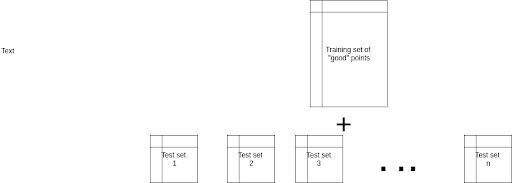
\includegraphics[width=1\columnwidth]{figures/rank_split.png}
    \caption{Validation setup for testing}
    \label{Validation setup for testing}
\end{figure*}

The learning set is further split into one combined training set and individual testing sets with 1 per each system of equations. This can be visualized by figure \ref{Validation setup for testing}, which is the setup used to validate the experiment. After, classification and before predictive modeling, experiments that are tagged "good" make up 85\% of the training set while the rest is made up of "bad" experiments. The selection of good experiments for training is made in random.

The idea behind having a training set dominated by "good" experiments is that it is a lot harder to predict those experiments since the execution times are to the power of -5 or lesser. This means even the slightest of inaccuracies can lead to drastic speed downs. On the other hand, "bad" experiments are to the power of -3, thereby reducing the impact of slight inaccuracies making it much easy to predict.

To make sure the model isn't over-fitting to "good" experiments, we made the testing sets entirely with "bad" experiments and just a single "good" experiment. Although in reality, one would rarely encounter a system of equation with only the choice of bad solvers, we wanted to simulate how the ranking framework performs in the worst conditions. 













